\section{Esempio di grafo reale}
Per analizzare meglio il sistema Bitcoin, viene creato un grafo delle transazioni, utilizzando dei dati reali. Nella \textit{figura \ref{fig:txgraph}} è visualizzato il grafo generato dall'elaborazione solo di 5 blocchi, in particolare dal blocco \textit{\#417113} al \textit{\#417117}.

\begin{figure}[htbp]
	\centering
	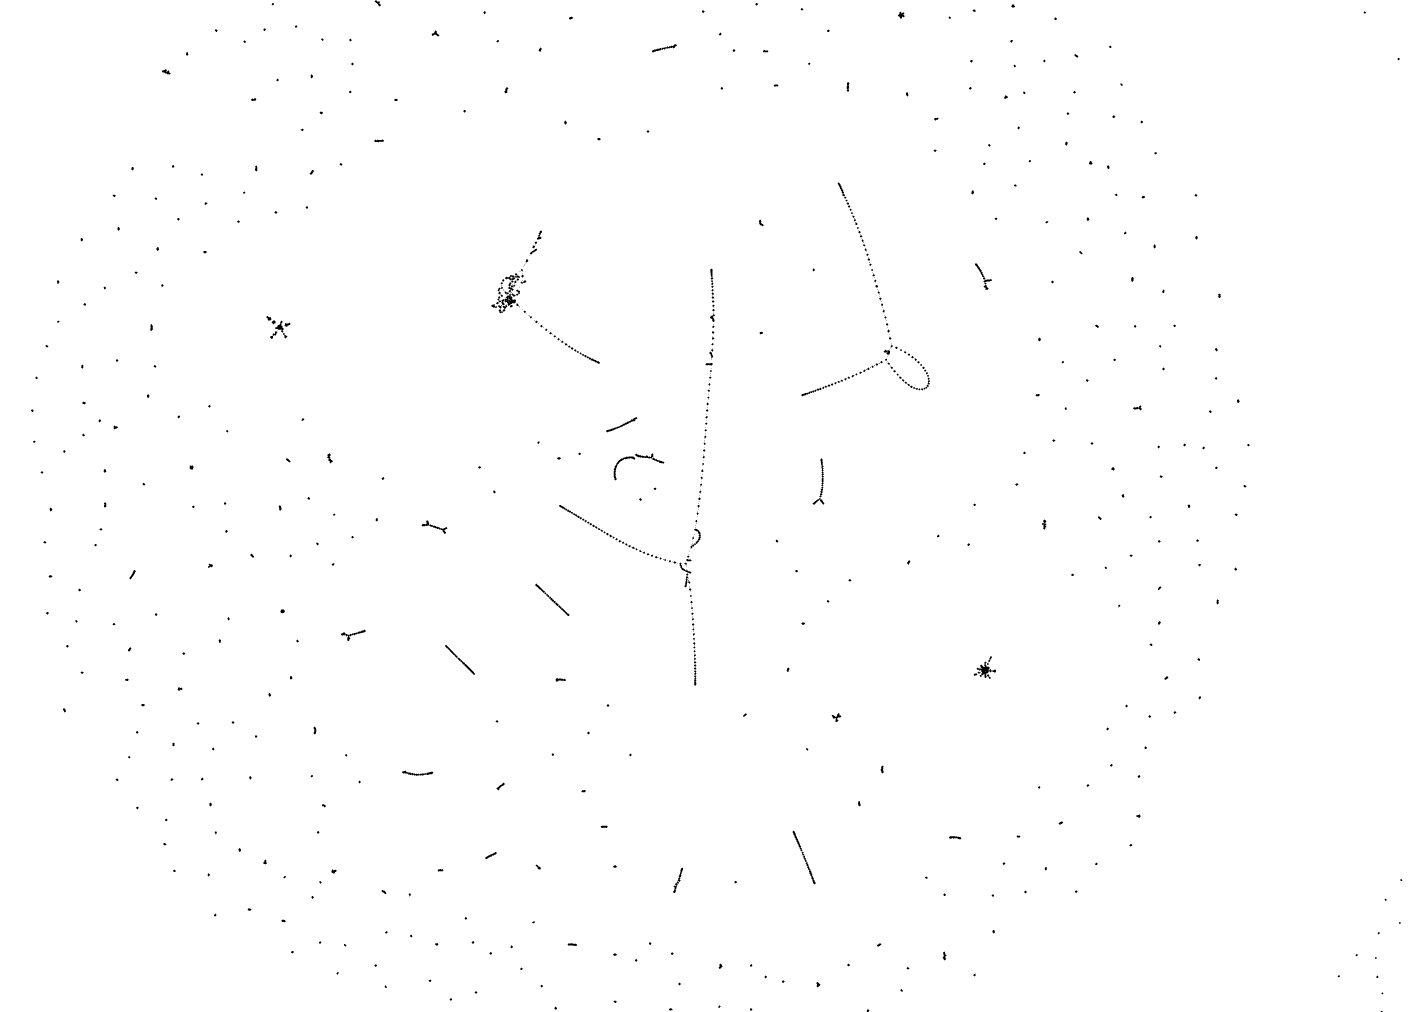
\includegraphics[width =0.8 \linewidth]{figure/txgraph}
	\caption{\textit{Esempio di tx-graph reale}}\label{fig:txgraph}
\end{figure}

Tale grafo viene visualizzato utilizzando il metodo \textit{force-directed}, ovvero assegnando ad ogni arco delle forze attrattive in modo da disporre i nodi del grafo.
A colpo d'occhio, al centro dell'immagine si notano alcune linee, che rappresentano delle sequenze di nodi collegati tra loro uno dopo l'altro.
Guardando man mano verso l'esterno, si notano molti nodi scollegati dal grafo: molto probabilmente rappresentano transazioni i cui output non sono stati spesi in transazioni incluse nell'intervallo di blocchi considerato, oppure che non sono stati spesi affatto.

\section{Lunghe catene di transazioni}
La media del numero di transazioni Bitcoin giornaliere è all'incirca 280'000, valutato a Maggio 2017. Questo numero è conosciuto per essere largamente influenzato da alcuni fenomeni.
Il mescolamento dei wallets e il mixing dei soldi sono solamente due esempi di attività che generano transazioni le quali non sono direttamente collegate con il reale acquisto di beni o servizi. Un altro esempio viene dall'attività di alcuni \textit{exchange}(organizzazioni che permettono agli utenti di scambiare Bitcoin per la valuta legale e viceversa) che usano lunghe catene di transazioni per emettere pagamenti verso degli utenti che hanno deciso di ritirare i Bitcoin. 

Questo tipo di organizzazioni aggregano diversi depositi di bitcoin dentro una singola grande transazione.  Sebbene tali catene di transazioni vengono innescate da attività umane (per esempio utenti che decidono di scambiare bitcoin), esse sono comunque generate da un meccanismo automatico, il quale incrementa il numero giornaliero delle transazioni associate al commercio esplicito di beni o servizi tra utenti.

Sulla base di ciò, si pensa che le organizzazioni con interessi sui Bitcoin, generano transazioni con il mero obiettivo di attrarre investitori e incrementare il tasso di scambio. Essendo generate da software, queste transazioni "artificiali" spesso introducono dei pattern regolari all'interno della Blockchain. E tali pattern vengono generati proprio perchè le catene di transazioni sono generate da un software programmato. 

Queste considerazioni vengono trattate approfonditamente nel paper \cite{ddp-ltcbh-17}. L'argomento principale di tale documento è il parametro \textit{LLC}, acronimo di \textit{lenght of the longest chain}, ovvero "lunghezza della catena più lunga". Ogni transazione viene etichettata con un LLC, ovvero un numero che rappresenta la catena più lunga a cui appartiene la transazione. Per assegnare questo parametro, viene precedentemente effettuata un'analisi sul grafo delle transazioni. Quindi, per ogni transazione, ovvero per ogni nodo, viene calcolato l'LLC e assegnato alla singola transazione. Infine vengono fatte delle analisi sui dati e sulla distribuzione del parametro rispetto ai blocchi considerati nell'esecuzione dell'algoritmo.

Capire se una chain di transazioni è stata generata automaticamente o riflette una chain creata da acquisti reali di umani, è una sfida stimolante. Infatti, la \textit{chain of ownership} ("catena di proprietà") introduce naturalmente lunghe chain di transazioni nel tx-graph. Quello che non è naturale è la velocità con cui tali chain vengono generate. 

\section{Analisi sul tx-graph}
 
Per effettuare analisi sul grafo delle transazioni, si è pensato di considerare dei parametri fondamentali nello studio di un fenomeno periodico come l'emissione di transazioni automatiche: la frequenza e la varianza.

Dal momento che le transazioni automatiche sono, molto spesso, generate a velocità elevata, si pensa di dare un parametro che quantizzi tale velocità. Tale parametro potrebbe essere la frequenza, ovvero quante transazioni vengono emesse nell'unità di tempo. 

Così facendo si potrebbe analizzare la frequenza delle singole catene di transazioni e dedurre quali sono quelle automatiche e non. Purtroppo, non si sa ancora in base a quale regola tali chain possono essere classificate. Si pensa soprattutto che questa analisi possa dare un contributo alla scoperta di nuovi andamenti.

Un altro parametro definito per l'analisi del grafo, è la varianza, ovvero la misura di quanto ci si discosta dalla media delle frequenze. Sebbene, la varianza debba essere calcolata istantaneamente, e la frequenza globalmente, si può fare una analisi "online". Infatti, man mano che si visita il grafo topologicamente e si scoprono nuove chain, si può calcolare la frequenza della chain fino alla transazione corrente, poi si calcola la varianza, e si potrebbe scegliere il cammino più lungo a varianza minima. In questo modo si potrebbe trovare una catena di transazioni generata automaticamente.

Dell'approccio utilizzato se ne parlerà nel capitolo 3.

\section{Frequenza delle transazioni}

Dal momento che tali catene di transazioni vengono generate automaticamente, esse vengono emesse ad una velocità elevata. Come si è già sottolineato nel capitolo precedente, un bitcoin mixer prende in input l'importo in bitcoin, l'indirizzo di destinazione e il tempo di ritardo con cui si vogliono ricevere tali bitcoin. In base al tempo inserito, il mixer creerà una certa quantità di transazioni collegate; più è maggiore il tempo, più transazioni verranno emesse, più è minore, meno si otterrà un anonimato su tali bitcoin.

Proprio per questo motivo, il mixer impiegherà una certa quantità di tempo per creare le transazioni che mischiano i bitcoin. Essendo un software programmato, esso genera le transazioni velocemente e ad intervalli regolari. Perciò, le catene generate da un mixer in modo automatico, verranno emesse in modo molto rapido ed ogni transazione di tali catene risulterà essere alla stessa distanza di tempo tra la sua precedente (se è presente) e la sua successiva nella catena.

Nella \textit{figura \ref{fig:zoomchain}} si osserva lo zoom su una catena del grafo di pagina \pageref*{fig:txgraph}.

\begin{figure}[htbp]
	\centering
	\begin{subfigure}[b]{0.4\textwidth}
		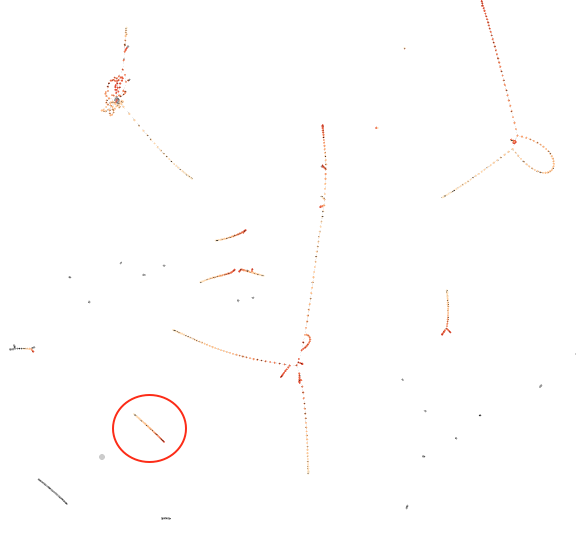
\includegraphics[width=\textwidth]{figure/zoomchain1}
		\caption{tx-graph}
		\label{fig:zoomchain1}
	\end{subfigure}\quad \qquad
	%add desired spacing between images, e. g. ~, \quad, \qquad, \hfill etc. 
	%(or a blank line to force the subfigure onto a new line)
	\begin{subfigure}[b]{0.4 \textwidth}
		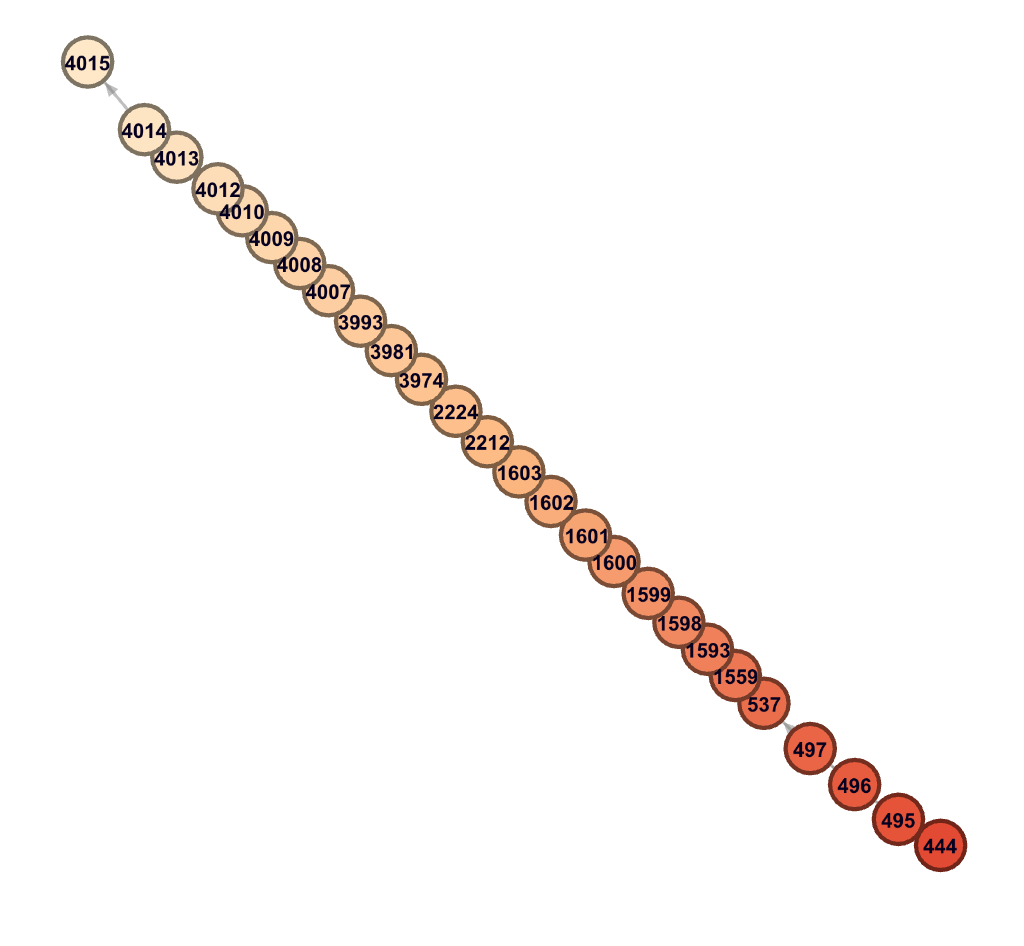
\includegraphics[width=\textwidth]{figure/zoomchain2}
		\caption{chain}
		\label{fig:zoomchain2}
	\end{subfigure}
	\caption{\textit{Zoom di una chain}}\label{fig:zoomchain}
\end{figure}

Dal momento che le chain vengono generate ad un'elevata velocità, si può pensare allo studio della densità temporale di tali transazioni. A partire da queste considerazioni, si può definire il concetto di \textbf{frequenza}.

La frequenza $f_T$ tra le $n$ transazioni $t_0,\cdots,t_n$, perciò, viene definita nella formula \ref{eq:freqtot}.
\begin{equation}
\centering
f_T = \frac{n}{ts(t_n) - ts(t_0)}
\label{eq:freqtot}
\end{equation}
Dove $f_T$ è la frequenza totale tra un numero $n$ di transazioni. $ts(t_0)$ è il timestamp della transazione iniziale $t_0$, mentre $ts(t_n)$ è il timestamp dell'ennesima transazione $t_n$. Tramite questa formula si ottiene la frequenza totale delle transazioni emesse in un certo intervallo di tempo.

Il concetto di frequenza totale, deriva dal concetto di frequenza fisica. Si definisca la \textbf{frequenza istantanea} come:
\begin{equation}
\centering
f_{ist}(t_n) = \frac{1}{T}
\quad con \quad
T = ts(t_n) - ts(t_{n-1})
\label{eq:freqist}
\end{equation}

La definizione di frequenza istantanea viene ripresa da quella della frequenza in fisica. In fisica la frequenza di un fenomeno, viene data dal numero degli eventi che vengono ripetuti in una data unità di tempo. L'unità di tempo $T$ in fisica è chiamata periodo, ed è l'intervallo temporale tra due eventi.

Nel caso del tx-graph, gli eventi sono le transazioni, e il periodo è calcolato tramite la differenza tra il timestamp dell'ultima transazione e quello della transazione iniziale, come si può notare nell'equazione \ref{eq:freqist}. La frequenza istantanea rappresenta il singolo valore di frequenza calcolato su due transazioni e su un singolo intervallo di tempo. Tale parametro non ha un ruolo significativo, se viene considerato a sè stante. Esso può essere inserito come parte della formula del calcolo della frequenza totale $f_T$. 

Nell'equazione \ref{eq:freqtot} la frequenza totale viene rappresentata come il rapporto tra la cardinalità delle transazioni diviso l'intervallo totale di tempo, ovvero il tempo che intercorre tra la transazione iniziale e quella finale. Allo stesso modo, se si riscrive la formula tenendo conto della media delle frequenze istantanee si otterrà:


\begin{eqnarray}
	f_T = \frac{f_{ist}(t_1)+\cdots+f_{ist}(t_n)}{n} = \label{eq:freqriga1} \\[20pt]
	= \left( \frac{1}{ts(t_1) - ts(t_0)}+\cdots+\frac{1}{ ts(t_n) - ts(t_{n-1})} \right) \cdot \frac{1}{n} = \label{eq:freqriga2}\\[20pt]
	= \frac{n}{( ts(t_1) - ts(t_0))+\cdots+(ts(t_n) - ts(t_{n-1}) )} \label{eq:freqriga3}
\end{eqnarray}
\\
dove il denominatore dell'equazione alla riga \ref{eq:freqriga3} è la somma di tutti i singoli intervalli di tempo tra le transazioni $t_0$ e $t_n$. Empiricamente, da tale somma si ottiene quindi l'intero intervallo di tempo tra la prima e l'ultima transazione, quindi il periodo totale sarà pari a $ts(t_n) - ts(t_0)$. 

L'equazione al punto \ref{eq:freqriga3} si può scrivere:

\begin{equation}
	f_T =  \frac{n}{ts(t_n) - ts(t_0)}
	\label{eq:freqfinal}
\end{equation}

Quindi, si ottiene la formula \ref{eq:freqtot} di pagina \pageref{eq:freqtot}. Sebbene le formule di frequenza totale e istantanea siano diverse tra loro, concatenando le varie frequenze istantanee si può arrivare a ottenere la formula $f_T$. 

Tutto ciò, al fine di sottolineare come la frequenza influenzi lo studio e l'analisi del grafo delle transazioni. Per ogni singola catena di transazioni viene calcolata la frequenza media tramite la formula \ref{eq:freqfinal}. Dalla frequenza, viene estrapolato un ulteriore parametro, la varianza, di cui si tratterà nella successiva sezione.

\section{Varianza}
Per analizzare meglio il grafo delle transazioni viene introdotto un ulteriore parametro la \textbf{varianza}, che dipende direttamente dalla frequenza. 
La nozione di varianza viene ripresa dalla nozione di varianza statistica. infatti per definizione la varianza fornisce una misura della variabilità dei valori assunti da una certa variabile, ovvero di quanto i valori di tale variabile si discostino dalla loro media aritmetica. \cite{wiki:varianza}

Dal punto di vista statistico, la varianza viene calcolata come la media quadratica dei discostamenti delle variabili prese in considerazione con la media aritmetica delle variabili stesse. Più generalmente la varianza va a misurare la variazione di un certo parametro rispetto al suo andamento medio.

Per adattare il concetto di varianza allo studio del tx-graph, si è deciso di utilizzare la formula \ref{eq:var} per il calcolo della varianza.

\begin{equation}
v =  \frac{ \sum_{i=1}^n (f_{ist}(t_i) - \mu )^2 }{n}
\label{eq:var}
\end{equation}

In questa formula, al denominatore è presente una sommatoria che sta a significare la somma delle varie quantità $f_{ist}(t_i) - \mu$ cioè i singoli discostamenti delle frequenze istantanee dalla media $\mu$.

La media infatti può essere calcolata con la formula standard della media aritmetica, sulle frequenze istantanee, ottenendo così:
\begin{equation}
	\mu = \frac{\sum_{i=1}^{n} f_{ist}(t_i)}{n}
\end{equation}

Gli studi che sono stati effettuati sul grafo delle transazioni, hanno tutti alla base queste nozioni di matematica. Infatti, la varianza viene calcolata in base alle frequenze istantanee, e quest'ultime vengono calcolate attraverso i timestamp delle singole transazioni. Le singole $f_{ist}$ rappresentano la frequenza con cui viene emessa una transazione, ovvero l'intervallo di tempo con cui una singola transazione viene effettuata. In questo modo si può capire quanto velocemente è stata emessa, e se eventualmente superi una certa soglia, si potrebbe intuire che essa è stata generata automaticamente. Empiricamente si può dedurre che un mixer può generare transazioni a intervalli regolari e velocemente. L'intervallo regolare è possibilmente deducibile con il calcolo della varianza, poichè più la varianza è bassa, più è possibile che le frequenze seguino un andamento regolare, uguale all'andamento del valor medio, ovvero del valore che più esprime la regolarità di una variabile.